% Example 32: CNN Forward Pass
% A simple convolutional neural network processing an image.
% Data flows left-to-right through Conv, Pool, Conv, Pool, FC, Output layers.
% Parameter: \PARAM (progress through the network, 0 to 1)
% Range: 0 to 1, recommended 120 frames
% Difficulty: intermediate
% Features demonstrated: neural network visualization, data flow animation, layer diagrams
\documentclass[tikz]{standalone}
\usepackage{tikz}
\usepackage{xcolor}
\usetikzlibrary{calc, positioning, arrows.meta}

% Brand Colors
\definecolor{garnet}{HTML}{73000A}
\definecolor{rose}{HTML}{CC2E40}
\definecolor{atlantic}{HTML}{466A9F}
\definecolor{congaree}{HTML}{1F414D}
\definecolor{horseshoe}{HTML}{65780B}
\definecolor{grass}{HTML}{CED318}
\definecolor{honeycomb}{HTML}{A49137}
\definecolor{warmgrey}{HTML}{676156}
\definecolor{sandstorm}{HTML}{FFF2E3}

% Fallback so the file compiles standalone (tikzgif replaces \PARAM)
\ifdefined\PARAM\else\def\PARAM{0.5}\fi

\begin{document}
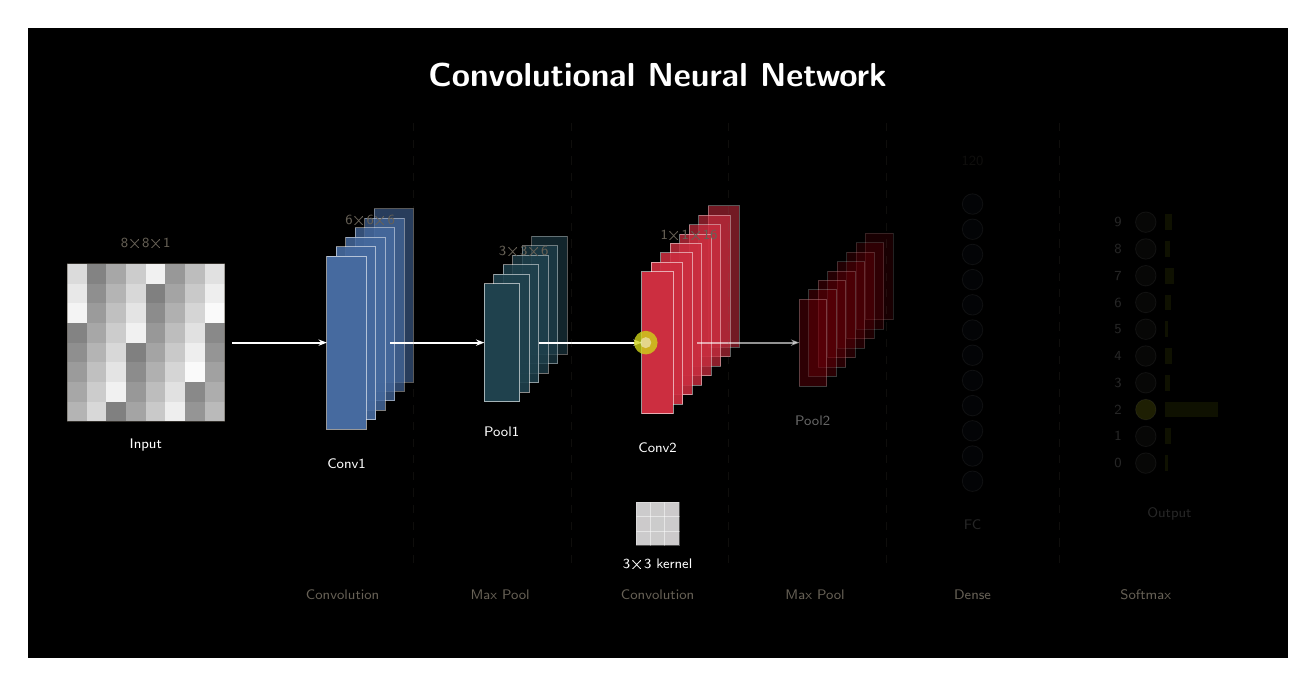
\begin{tikzpicture}
  \useasboundingbox (-8,-4) rectangle (8,4);

  % Animation parameter: 0 to 1
  \pgfmathsetmacro{\t}{\PARAM}

  % ====== Background ======
  \fill[black] (-8,-4) rectangle (8,4);

  % ====== Title ======
  \node[white, font=\sffamily\bfseries\large] at (0, 3.4) {Convolutional Neural Network};

  % ====== Layer x-positions ======
  % Input | Conv1 | Pool1 | Conv2 | Pool2 | Flatten | FC | Output
  \def\xInput{-6.5}
  \def\xConvA{-4.2}
  \def\xPoolA{-2.2}
  \def\xConvB{-0.2}
  \def\xPoolB{1.8}
  \def\xFC{4.0}
  \def\xOut{6.2}

  % ====== Progress thresholds for each layer ======
  % t in [0, 1] maps to data arriving at each stage
  \pgfmathsetmacro{\tConvA}{0.14}
  \pgfmathsetmacro{\tPoolA}{0.28}
  \pgfmathsetmacro{\tConvB}{0.42}
  \pgfmathsetmacro{\tPoolB}{0.56}
  \pgfmathsetmacro{\tFC}{0.72}
  \pgfmathsetmacro{\tOut}{0.86}

  % ====== Helper: feature map block (stacked rectangles with 3D offset) ======
  % #1=x, #2=width, #3=height, #4=depth layers, #5=color, #6=opacity
  \newcommand{\featuremap}[6]{%
    \foreach \k in {1,...,#4}{%
      \pgfmathsetmacro{\ox}{0.12*(#4-\k)}%
      \pgfmathsetmacro{\oy}{0.12*(#4-\k)}%
      \pgfmathsetmacro{\myopac}{#6 * (0.5 + 0.5*\k/#4)}%
      \fill[#5, opacity=\myopac]
        ({#1+\ox},{-#3/2+\oy}) rectangle ({#1+#2+\ox},{#3/2+\oy});
      \draw[white, opacity={\myopac*0.6}, line width=0.3pt]
        ({#1+\ox},{-#3/2+\oy}) rectangle ({#1+#2+\ox},{#3/2+\oy});
    }%
  }

  % ====== Activation glow helper ======
  % Opacity of each layer based on whether data has arrived
  \pgfmathsetmacro{\opInput}{1.0}
  \pgfmathsetmacro{\opConvA}{min(1.0, max(0.15, (\t - \tConvA + 0.1) / 0.1))}
  \pgfmathsetmacro{\opPoolA}{min(1.0, max(0.15, (\t - \tPoolA + 0.1) / 0.1))}
  \pgfmathsetmacro{\opConvB}{min(1.0, max(0.15, (\t - \tConvB + 0.1) / 0.1))}
  \pgfmathsetmacro{\opPoolB}{min(1.0, max(0.15, (\t - \tPoolB + 0.1) / 0.1))}
  \pgfmathsetmacro{\opFC}{min(1.0, max(0.15, (\t - \tFC + 0.1) / 0.1))}
  \pgfmathsetmacro{\opOut}{min(1.0, max(0.15, (\t - \tOut + 0.1) / 0.1))}

  % ====== Draw layers ======

  % --- Input image (8x8 pixel grid) ---
  \begin{scope}[shift={(\xInput, 0)}]
    \def\gs{0.25}  % grid cell size
    \def\gn{8}     % grid count
    \pgfmathsetmacro{\gw}{\gs*\gn}
    % Draw pixel grid with pseudo-random grayscale values
    \foreach \r in {0,...,7}{
      \foreach \c in {0,...,7}{
        \pgfmathsetmacro{\val}{50 + mod(\r*37 + \c*53 + 17, 41)*1.2}
        \fill[white!\val!black, opacity=\opInput]
          ({\c*\gs - \gw/2},{\r*\gs - \gw/2}) rectangle
          ({(\c+1)*\gs - \gw/2},{(\r+1)*\gs - \gw/2});
      }
    }
    \draw[warmgrey, opacity=0.5, line width=0.3pt]
      ({-\gw/2},{-\gw/2}) rectangle ({\gw/2},{\gw/2});
    \node[white, font=\sffamily\tiny, below] at (0, {-\gw/2 - 0.1}) {Input};
    \node[warmgrey, font=\sffamily\tiny, above] at (0, {\gw/2 + 0.05}) {8\texttimes8\texttimes1};
  \end{scope}

  % --- Conv1: 6 feature maps, 6x6 ---
  \featuremap{\xConvA}{0.5}{2.2}{6}{atlantic}{\opConvA}
  \node[white, font=\sffamily\tiny, below, opacity=\opConvA] at ({\xConvA+0.25}, -1.35) {Conv1};
  \node[warmgrey, font=\sffamily\tiny, above, opacity=\opConvA] at ({\xConvA+0.55}, 1.35) {6\texttimes6\texttimes6};

  % --- Pool1: 6 feature maps, 3x3 ---
  \featuremap{\xPoolA}{0.45}{1.5}{6}{congaree}{\opPoolA}
  \node[white, font=\sffamily\tiny, below, opacity=\opPoolA] at ({\xPoolA+0.22}, -0.95) {Pool1};
  \node[warmgrey, font=\sffamily\tiny, above, opacity=\opPoolA] at ({\xPoolA+0.5}, 0.95) {3\texttimes3\texttimes6};

  % --- Conv2: 16 feature maps, 1x1 (small) ---
  \featuremap{\xConvB}{0.4}{1.8}{8}{rose}{\opConvB}
  \node[white, font=\sffamily\tiny, below, opacity=\opConvB] at ({\xConvB+0.2}, -1.15) {Conv2};
  \node[warmgrey, font=\sffamily\tiny, above, opacity=\opConvB] at ({\xConvB+0.6}, 1.15) {1\texttimes1\texttimes16};

  % --- Pool2: 16 feature maps, smaller ---
  \featuremap{\xPoolB}{0.35}{1.1}{8}{garnet}{\opPoolB}
  \node[white, font=\sffamily\tiny, below, opacity=\opPoolB] at ({\xPoolB+0.17}, -0.8) {Pool2};

  % --- Fully Connected layer (vertical column of neurons) ---
  \begin{scope}[shift={(\xFC, 0)}]
    \def\nFC{12}
    \pgfmathsetmacro{\spacingFC}{0.32}
    \foreach \i in {1,...,\nFC}{
      \pgfmathsetmacro{\ny}{(\i - (\nFC+1)/2) * \spacingFC}
      \pgfmathsetmacro{\pulse}{(\t > \tFC) ? (0.4 + 0.6*sin(mod(\i*60 + \t*720, 360))) : 0.3}
      \pgfmathsetmacro{\nopac}{\opFC * \pulse}
      \fill[atlantic, opacity=\nopac] (0, \ny) circle (0.13);
      \draw[white, opacity={\opFC*0.4}, line width=0.3pt] (0, \ny) circle (0.13);
    }
    \node[white, font=\sffamily\tiny, below, opacity=\opFC] at (0, {-(\nFC+1)/2*\spacingFC - 0.05}) {FC};
    \node[warmgrey, font=\sffamily\tiny, above, opacity=\opFC] at (0, {(\nFC+1)/2*\spacingFC + 0.05}) {120};
  \end{scope}

  % --- Output layer (10 class neurons) ---
  \begin{scope}[shift={(\xOut, 0)}]
    \def\nOut{10}
    \pgfmathsetmacro{\spacingOut}{0.34}
    % Determine "winning" class
    \pgfmathtruncatemacro{\winClass}{3}  % class 3 wins
    \foreach \i in {1,...,\nOut}{
      \pgfmathsetmacro{\ny}{(\i - (\nOut+1)/2) * \spacingOut}
      \pgfmathsetmacro{\isWinner}{(\i == \winClass) ? 1 : 0}
      \pgfmathsetmacro{\classConf}{(\isWinner > 0.5) ? 0.95 : (0.05 + 0.12*mod(\i*7+3,5)/5)}
      \pgfmathsetmacro{\barW}{0.7 * \classConf}
      \pgfmathsetmacro{\barOpac}{\opOut}
      % Confidence bar
      \fill[horseshoe, opacity=\barOpac]
        (0.25, {\ny - 0.1}) rectangle ({0.25 + \barW}, {\ny + 0.1});
      % Neuron
      \pgfmathsetmacro{\ncol}{(\isWinner > 0.5) ? 1 : 0}
      \ifnum\ncol=1
        \fill[grass, opacity=\barOpac] (0, \ny) circle (0.13);
      \else
        \fill[warmgrey, opacity={\barOpac*0.5}] (0, \ny) circle (0.13);
      \fi
      \draw[white, opacity={\barOpac*0.4}, line width=0.3pt] (0, \ny) circle (0.13);
      % Class label
      \pgfmathtruncatemacro{\classLabel}{\i - 1}
      \node[white, font=\sffamily\tiny, opacity=\barOpac, left] at (-0.18, \ny) {\classLabel};
    }
    \node[white, font=\sffamily\tiny, below, opacity=\opOut] at (0.3, {-(\nOut+1)/2*\spacingOut - 0.1}) {Output};
  \end{scope}

  % ====== Data flow arrows between layers ======
  \newcommand{\flowarrow}[3]{%
    % #1=x_start, #2=x_end, #3=progress opacity
    \pgfmathsetmacro{\arrowopac}{#3}%
    \draw[-{Stealth[length=3pt]}, white, opacity=\arrowopac, line width=0.8pt]
      (#1, 0) -- (#2, 0);
  }

  % Compute arrow opacities based on data flow progress
  \pgfmathsetmacro{\arA}{min(1.0, max(0.0, (\t) / \tConvA))}
  \pgfmathsetmacro{\arB}{min(1.0, max(0.0, (\t - \tConvA) / (\tPoolA - \tConvA)))}
  \pgfmathsetmacro{\arC}{min(1.0, max(0.0, (\t - \tPoolA) / (\tConvB - \tPoolA)))}
  \pgfmathsetmacro{\arD}{min(1.0, max(0.0, (\t - \tConvB) / (\tPoolB - \tConvB)))}
  \pgfmathsetmacro{\arE}{min(1.0, max(0.0, (\t - \tPoolB) / (\tFC - \tPoolB)))}
  \pgfmathsetmacro{\arF}{min(1.0, max(0.0, (\t - \tFC) / (\tOut - \tFC)))}

  % Draw flow arrows
  \flowarrow{-5.4}{-4.2}{\arA}    % Input -> Conv1
  \flowarrow{-3.4}{-2.2}{\arB}    % Conv1 -> Pool1
  \flowarrow{-1.5}{-0.2}{\arC}    % Pool1 -> Conv2
  \flowarrow{0.5}{1.8}{\arD}      % Conv2 -> Pool2
  \flowarrow{2.5}{3.8}{\arE}      % Pool2 -> FC
  \flowarrow{4.2}{5.9}{\arF}      % FC -> Output

  % ====== Animated data pulse ======
  % A bright dot moving along the data path
  \pgfmathsetmacro{\pulseX}{-6.5 + \t * 12.7}
  \pgfmathsetmacro{\pulseOpac}{0.8 * (1 - abs(2*\t - 1))}
  \fill[grass, opacity=\pulseOpac] (\pulseX, 0) circle (0.15);
  \fill[white, opacity={\pulseOpac*0.6}] (\pulseX, 0) circle (0.07);

  % ====== Kernel visualization (during conv stages) ======
  % Show a small 3x3 kernel near active conv layer
  \pgfmathsetmacro{\showKernelA}{(\t > 0.02) && (\t < \tPoolA) ? 1 : 0}
  \ifnum\showKernelA=1
    \begin{scope}[shift={(\xConvA + 0.25, -2.3)}]
      \def\ks{0.18}
      \foreach \kr in {0,1,2}{
        \foreach \kc in {0,1,2}{
          \pgfmathsetmacro{\kval}{mod(\kr*3+\kc+2, 5) / 5}
          \fill[atlantic!\kval!white, opacity=0.8]
            ({\kc*\ks - 1.5*\ks},{\kr*\ks - 1.5*\ks}) rectangle
            ({(\kc+1)*\ks - 1.5*\ks},{(\kr+1)*\ks - 1.5*\ks});
          \draw[white, opacity=0.3, line width=0.2pt]
            ({\kc*\ks - 1.5*\ks},{\kr*\ks - 1.5*\ks}) rectangle
            ({(\kc+1)*\ks - 1.5*\ks},{(\kr+1)*\ks - 1.5*\ks});
        }
      }
      \node[white, font=\sffamily\tiny, below] at (0, {-1.5*\ks - 0.05}) {3\texttimes3 kernel};
    \end{scope}
  \fi

  \pgfmathsetmacro{\showKernelB}{(\t > \tPoolA) && (\t < \tPoolB) ? 1 : 0}
  \ifnum\showKernelB=1
    \begin{scope}[shift={(\xConvB + 0.2, -2.3)}]
      \def\ks{0.18}
      \foreach \kr in {0,1,2}{
        \foreach \kc in {0,1,2}{
          \pgfmathsetmacro{\kval}{mod(\kr*2+\kc+1, 4) / 4}
          \fill[rose!\kval!white, opacity=0.8]
            ({\kc*\ks - 1.5*\ks},{\kr*\ks - 1.5*\ks}) rectangle
            ({(\kc+1)*\ks - 1.5*\ks},{(\kr+1)*\ks - 1.5*\ks});
          \draw[white, opacity=0.3, line width=0.2pt]
            ({\kc*\ks - 1.5*\ks},{\kr*\ks - 1.5*\ks}) rectangle
            ({(\kc+1)*\ks - 1.5*\ks},{(\kr+1)*\ks - 1.5*\ks});
        }
      }
      \node[white, font=\sffamily\tiny, below] at (0, {-1.5*\ks - 0.05}) {3\texttimes3 kernel};
    \end{scope}
  \fi

  % ====== Layer type labels along the bottom ======
  \node[warmgrey, font=\sffamily\tiny] at (-4.0, -3.2) {Convolution};
  \node[warmgrey, font=\sffamily\tiny] at (-2.0, -3.2) {Max Pool};
  \node[warmgrey, font=\sffamily\tiny] at (0.0, -3.2) {Convolution};
  \node[warmgrey, font=\sffamily\tiny] at (2.0, -3.2) {Max Pool};
  \node[warmgrey, font=\sffamily\tiny] at (4.0, -3.2) {Dense};
  \node[warmgrey, font=\sffamily\tiny] at (6.2, -3.2) {Softmax};

  % Thin separator lines
  \foreach \lx in {-3.1, -1.1, 0.9, 2.9, 5.1}{
    \draw[warmgrey, opacity=0.15, line width=0.3pt, dashed]
      (\lx, -2.8) -- (\lx, 2.8);
  }

\end{tikzpicture}
\end{document}
